\documentclass[border=5pt]{standalone}

\usepackage{tikz}
\usetikzlibrary{shapes.gates.logic.US}
\begin{document}

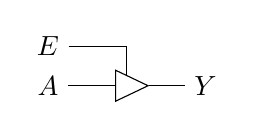
\begin{tikzpicture}
\node (A) at (0,0) {$A$};
\node (E) at (0,0.5) {$E$};
\node (Y) at (2,0) {$Y$};
\node[buffer gate US, draw, logic gate inputs=n] at (1,0) (TS) {};
\draw (A) -- (TS.input);
\draw (E) -| (TS.north);
\draw (TS.output) -- (Y);
\end{tikzpicture}

\end{document}
